\documentclass[10.5pt,]{article}

\usepackage{multicol} % for multiple columns



\usepackage[sc, osf]{mathpazo}
\usepackage{amssymb,amsmath}
\usepackage{ifxetex,ifluatex}
\usepackage{fixltx2e} % provides \textsubscript
\ifnum 0\ifxetex 1\fi\ifluatex 1\fi=0 % if pdftex
\usepackage[T1]{fontenc}
\usepackage[utf8]{inputenc}
\else % if luatex or xelatex
\ifxetex
\usepackage{xltxtra,xunicode} %originally, \usepackage{mathspec}. This change is to produce Chinese
\else
\usepackage{fontspec}
\fi
\defaultfontfeatures{Ligatures=TeX,Scale=MatchLowercase}
\fi
% use upquote if available, for straight quotes in verbatim environments
\IfFileExists{upquote.sty}{\usepackage{upquote}}{}
% use microtype if available
\IfFileExists{microtype.sty}{%
	\usepackage{microtype}
	\UseMicrotypeSet[protrusion]{basicmath} % disable protrusion for tt fonts
}{}
\usepackage[margin=1in]{geometry}




\setlength{\emergencystretch}{3em}  % prevent overfull lines
\providecommand{\tightlist}{%
	\setlength{\itemsep}{0pt}\setlength{\parskip}{0pt}}
\setcounter{secnumdepth}{0}
% Redefines (sub)paragraphs to behave more like sections
\ifx\paragraph\undefined\else
\let\oldparagraph\paragraph
\renewcommand{\paragraph}[1]{\oldparagraph{#1}\mbox{}}
\fi
\ifx\subparagraph\undefined\else
\let\oldsubparagraph\subparagraph
\renewcommand{\subparagraph}[1]{\oldsubparagraph{#1}\mbox{}}
\fi

% Now begins the stuff that I added.
% ----------------------------------

% Custom section fonts
\usepackage{sectsty}
\sectionfont{\rmfamily\mdseries\large\bf}
\subsectionfont{\rmfamily\mdseries\normalsize\itshape}


% Make lists without bullets
\renewenvironment{itemize}{
	\begin{list}{}{
			\setlength{\leftmargin}{1.5em}
		}
	}{
	\end{list}
}


% Make parskips rather than indent with lists.
\usepackage{parskip}
\usepackage{titlesec}

\usepackage{ctex}
% Siyuan Font
%\setCJKmainfont[BoldFont = Noto Sans CJK SC]{Noto Serif CJK SC}
%\setCJKsansfont{Noto Sans CJK SC}
%\setCJKfamilyfont{zhsong}{Noto Serif CJK SC}
%\setCJKfamilyfont{zhhei}{Noto Sans CJK SC}
%\setCJKfamilyfont{zhkai}{simkai.ttf}

% less space for the Chinese format
\titlespacing\section{0pt}{1pt plus 4pt minus 2pt}{1pt plus 2pt minus 2pt}
\titlespacing\subsection{0pt}{5pt plus 4pt minus 2pt}{0pt plus 2pt minus 2pt}


% Use fontawesome. Note: you'll need TeXLive 2015. Update.
\usepackage{fontawesome}
\newfontfamily\FA{FontAwesome.otf} % Explicitly provide .otf

% Fancyhdr, as I tend to do with these personal documents.
\usepackage{fancyhdr,lastpage}
\pagestyle{fancy}
\renewcommand{\headrulewidth}{0.0pt}
\renewcommand{\footrulewidth}{0.0pt}
\lhead{}
\chead{}
\rhead{}
\lfoot{
	\cfoot{\scriptsize  胡悦 - 教学简历 }}
\rfoot{\scriptsize \thepage/{\hypersetup{linkcolor=black}\pageref{LastPage}}}

% Always load hyperref last.
\usepackage{hyperref}
\PassOptionsToPackage{usenames,dvipsnames}{color} % color is loaded by hyperref

\hypersetup{unicode=true,
		pdftitle={胡悦:  教学简历 (Curriculum Vitae)},
			pdfauthor={胡悦},
			colorlinks=true,
	linkcolor=blue,
	citecolor=Blue,
	urlcolor=blue,
	breaklinks=true, bookmarks=true}
\urlstyle{same}  % don't use monospace font for urls

% try to fit picture
\usepackage{tikz}


\begin{document}
	
	
	\centerline{\huge \bf 胡悦}
	
	
	
	\vspace{2 mm}
	
	\hrule
	
	\vspace{2 mm}
	
	
	\moveleft.5\hoffset\centerline{北京市海淀区清华大学明斋114, 邮编:100084}
	\moveleft.5\hoffset\centerline{ {\FA\faEnvelope} \hspace{1 mm} \href{mailto:}{\tt \href{mailto:yue-hu-1@uiowa.edu}{\nolinkurl{yue-hu-1@uiowa.edu}}} \hspace{1 mm}     {\FA\faGlobe} \hspace{1 mm} \href{http://sammo3182.github.io}{\tt sammo3182.github.io}   }
	
	\vspace{2 mm}
	
	\hrule
	
		\begin{tikzpicture}[remember picture,overlay]
	\node[xshift=163mm,yshift=-4mm,anchor=north west] at (current page.north west){%
		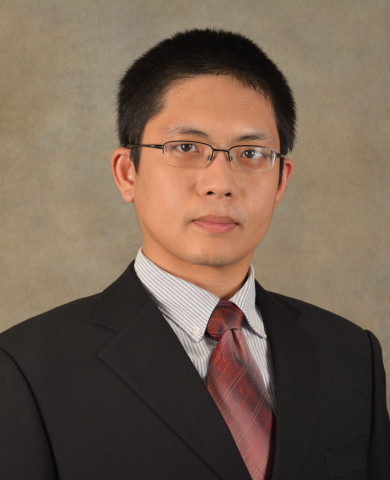
\includegraphics[width=28mm]{verticalYueHu.jpg}};
	\end{tikzpicture}
		
	\hypertarget{section}{%
\section{教学经历}\label{section}}

\begin{itemize}
\tightlist
\item
  爱荷华大学:
  任课教师(政治学研究设计、R语言与社会科学研究系列讲座),教学助理(比较政治学入门等)
\item
  南卡罗来纳大学:教学助理(国际关系学、争论中的世界政治、比较政治:发展中国家等)
\item
  里贾纳大学:教学助理(政治学入门)
\end{itemize}

\hypertarget{section-1}{%
\section{助教详情}\label{section-1}}

\hypertarget{university-of-iowa}{%
\subsection{University of Iowa}\label{university-of-iowa}}

\begin{itemize}
\tightlist
\item
  Introduction to Political Behavior\hfill Spring 2015
\item
  Introduction to International Relations\hfill Fall 2014
\item
  Introduction to Comparative Politics\hfill Spring 2014
\item
  Political Campaigning\hfill Fall 2014
\item
  Political Psychology\hfill Fall 2014
\end{itemize}

\hypertarget{university-of-south-carolina}{%
\subsection{University of South
Carolina}\label{university-of-south-carolina}}

\begin{itemize}
\tightlist
\item
  International Relations\hfill Spring 2013
\item
  Comparative Politics\hfill Spring 2013
\item
  Controversial World Politics\hfill Fall 2012
\item
  American National Government\hfill Spring 2012
\item
  Comparative Politics-Developing Countries\hfill Spring 2012
\item
  National Security of United States\hfill Fall 2011
\end{itemize}

\hypertarget{university-of-regina}{%
\subsection{University of Regina}\label{university-of-regina}}

\begin{itemize}
\tightlist
\item
  Introduction to Political Science\hfill Fall 2010
\end{itemize}

\hypertarget{section-2}{%
\section{教学技能}\label{section-2}}

\begin{itemize}
\tightlist
\item
  分析与编程: R, Stata, Python, C++, Mathematica, NetLogo, JAGS, UCINET
\item
  应用: \LaTeX, Markdown, Git(GitHub)
\end{itemize}
	
			\end{document}